\documentclass[11pt, a4paper]{article}
%\usepackage{proj1}
\usepackage{natbib}
\usepackage{fancyhdr}  
\usepackage{subcaption}
\usepackage{caption}
\usepackage{graphicx}
\linespread{1.25} 
\setlength{\parindent}{0cm}
\graphicspath{{Images/}}
\usepackage{hyperref}
\usepackage{amsmath}
\usepackage{amsfonts}
\usepackage{amssymb}
\usepackage{amsthm}
\usepackage{mathtools}
\usepackage{commath}

%\usepackage[sc,osf]{mathpazo}
\usepackage{subcaption}
\usepackage[a4paper, top=1in, left=1.0in, right=1.0in, bottom=1in, includehead, includefoot]{geometry} %Usually have top as 1in

\usepackage{listings}
\usepackage{color} %red, green, blue, yellow, cyan, magenta, black, white
\definecolor{mygreen}{RGB}{28,172,0} % color values Red, Green, Blue
\definecolor{mylilas}{RGB}{170,55,241}


\hypersetup{colorlinks,linkcolor={black},citecolor={blue},urlcolor={black}}
\usepackage{color}
\urlstyle{same}


\theoremstyle{definition}
\newtheorem{definition}{Definition}[section]

\title{Exact Solutions for the Full Problem \\with Force Control and with Flow Control}
\date{}
\newcommand{\Sta}{\rho}
\newcommand{\Adj}{p}
\newcommand{\Con}{u}

\pagenumbering{gobble}
\begin{document}
\section*{Report 23/04/2020 (Part 2)}
Note: all of the results are done with Picard, but most have been checked with FixPt and give the same qualitative answer (i.e. which parameter configurations converge and which don't).\\
Note 2: Can't get the $\rho = e^h$ approach to work. It gives 'singular matrices'. Forward Result looks fine, chose $\rho >1$ everywhere.
\section{Investigating the relationship between Diffusion and Advection}
We are looking at the exact flow control problem and perturb it in time by the standard bump function:
\begin{align*}
w_{Pert} = w_{Ex} (1 + 0.1\tilde g(t)).
\end{align*}
Then two cases are considered:\\
1. Choose an example that diverges and see if changing $D_0$ can make it converge.\\
2. Choose an example that converges and see if changing $D_0$ breaks it.\\
We choose the Picard solver, $\beta = 10^{-3}$, tolerances $10^{-8}/10^{-4}$ and $\lambda =0.1$.\\
For 2.:\\
Choosing scalerho, scalep $=1$ (the coefficient in front of $\rho_{IC}$ and $p_{IC}$), we have $\max \rho = 0.2576$, $\max p = 0.0543$ and $\max w = 12.7707$ (measured by 'max(max(abs))'). This converges in $246$ iterations.\\
For 1.:\\
Choosing scalerho, scalep $=2$, the algorithm diverges at $0.00033691$ at iteration $83$. The order of magnitude for the variables with this scaling are: $\max \rho = 0.5152$, $\max p = 0.1087$ and $\max w = 51.0827$. This shows that $w$ does not grow linearly with a linear scaling of $\rho$ and $p$ (as expected).

\subsection{Test 1: Fixing a diverging example}
Trying $D_0= 2$, the initial consistency error is $0.08751198$ (with $D_0 = 1$ it is $0.10321139$), so it decreased. However, the problem diverges at a consistency of $0.00038865$, which is earlier than with $D_0=1$. For $D_0=3$, the initial error is $0.07665870$ and it diverges at $0.00047412$, which is again earlier than with lower $D_0$. 
Setting $D_0 = 10$, the initial error is $0.03677095$. It diverges at $0.00043914$. I am not sure why convergence doesn't improve 'linearly' as we increase the diffusion.
Setting $D_0 = 20$, it diverges at $0.00023938$, which is going in the right direction.
Setting $D_0 = 50$, the initial error is $0.00733544$ and it converges in $72$ iterations. Given the difference in magnitude of $\rho$ and $w$ it is not so surprising that a large $D_0$ is needed, see Figure \ref{rhoD03}, compare to $D_0 = 1$ forward solution in Figure \ref{rhoD03a}. The lowest converging problem has diffusion coefficient $D_0 = 30$. This makes perfect sense because heuristically:
$\max \rho \simeq 1.5$ and 

\begin{figure}[h]
	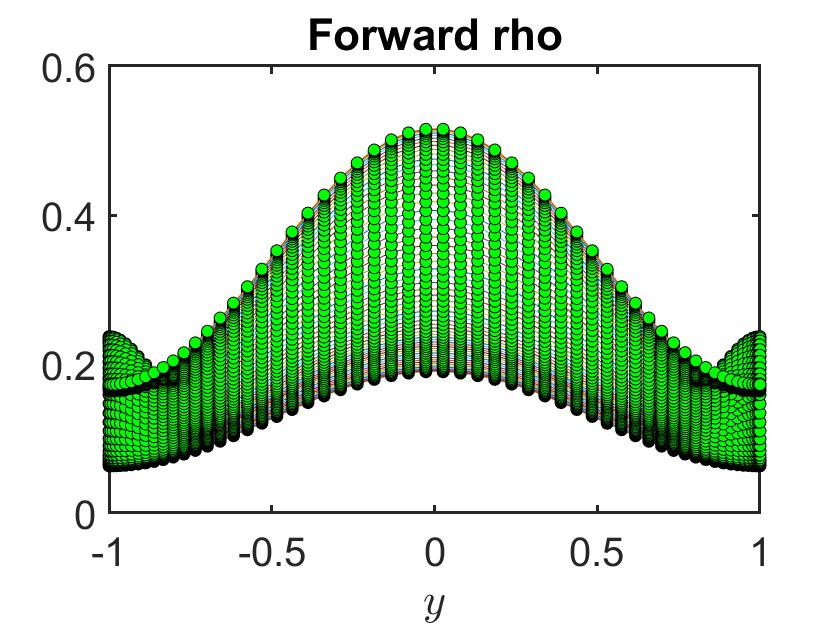
\includegraphics[scale=0.3]{wFrhoFW1a.jpg}	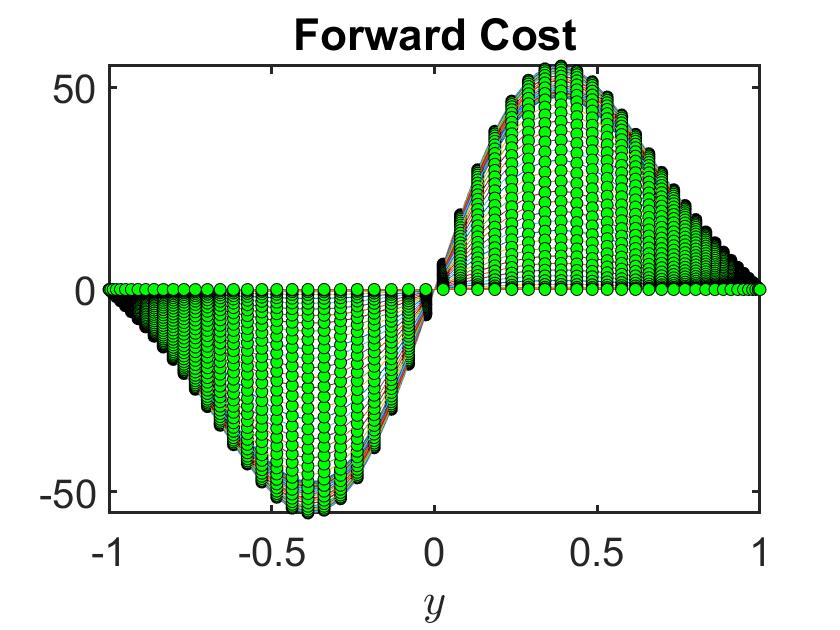
\includegraphics[scale=0.3]{wFwFW1a.jpg}
	\caption{Solutions $\rho_{FW}$ and $w_{FW}$,   with $D_0 = 1$.}
	\label{rhoD03a}
\end{figure}
\begin{figure}[h]
	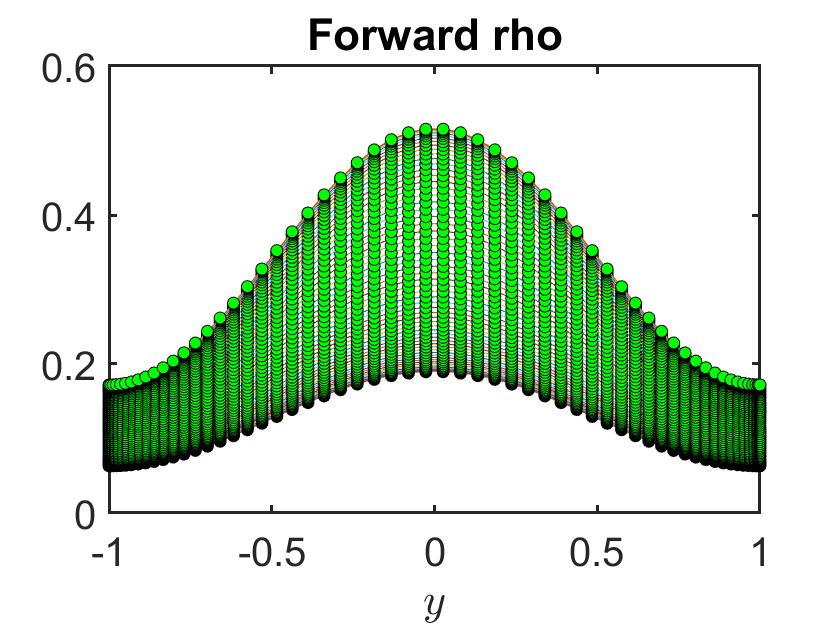
\includegraphics[scale=0.3]{wFrhoFW1.jpg}	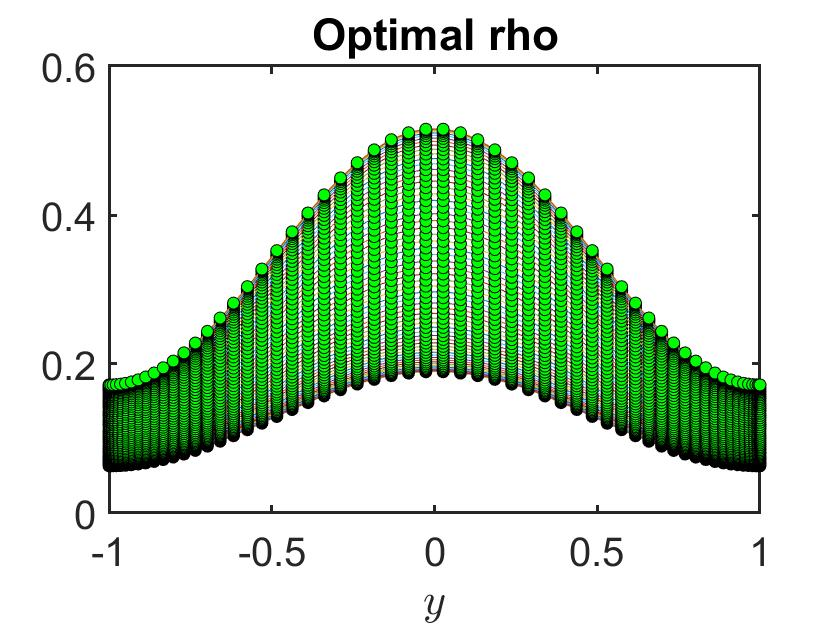
\includegraphics[scale=0.3]{wFrhoOpt1.jpg}
	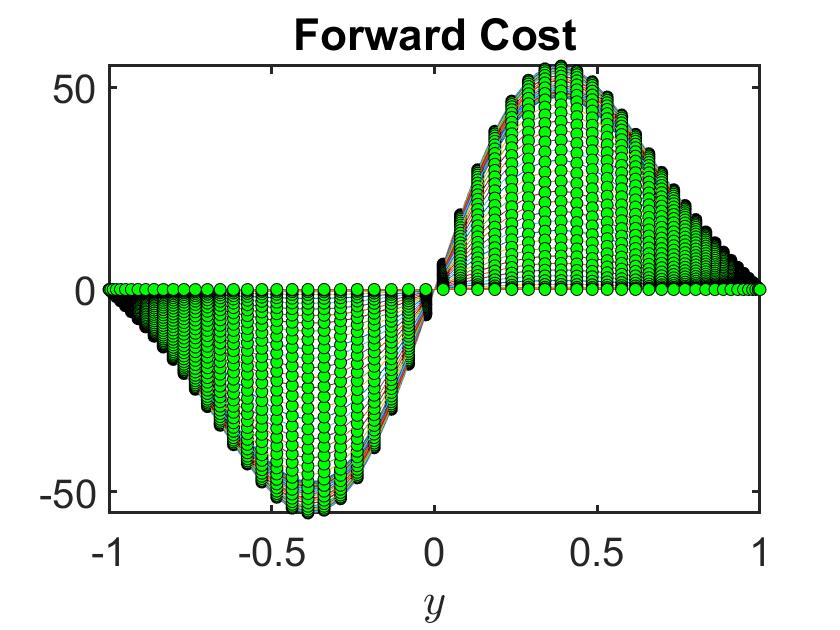
\includegraphics[scale=0.3]{wFwFW1.jpg}
	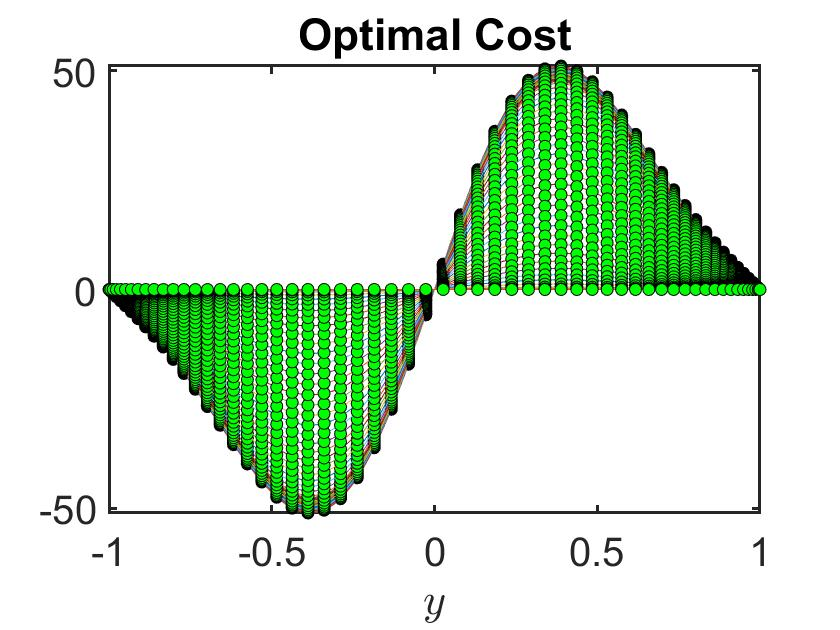
\includegraphics[scale=0.3]{wFwOpt1.jpg}
	\caption{Solutions $\rho_{FW}$ and $\rho_{Opt}$, $w_{FW}$ and $w_{Opt}$,   with $D_0 = 50$.}
	\label{rhoD03}
\end{figure}

\subsection{Test 2: Breaking a converging example}
Choose $\beta = 10^{-3}$, scalerho, scalep $=1$. This converges within $246$ iterations, see Figure \ref{rhoD032}. When choosing $D_0 = 0.5$ instead then it diverges at $0.00029311$ and with $D_0 = 0.1$ it diverges at $0.00433974$. The forward solution and cost for $D_0=0.1$ is displayed in Figure \ref{rhoD032a}. The behaviour of $\rho$ close to the boundary is very similar to the boundary in Figure \ref{rhoD03a}, which is the diverging problem in Test 1. 


\begin{figure}[h]
	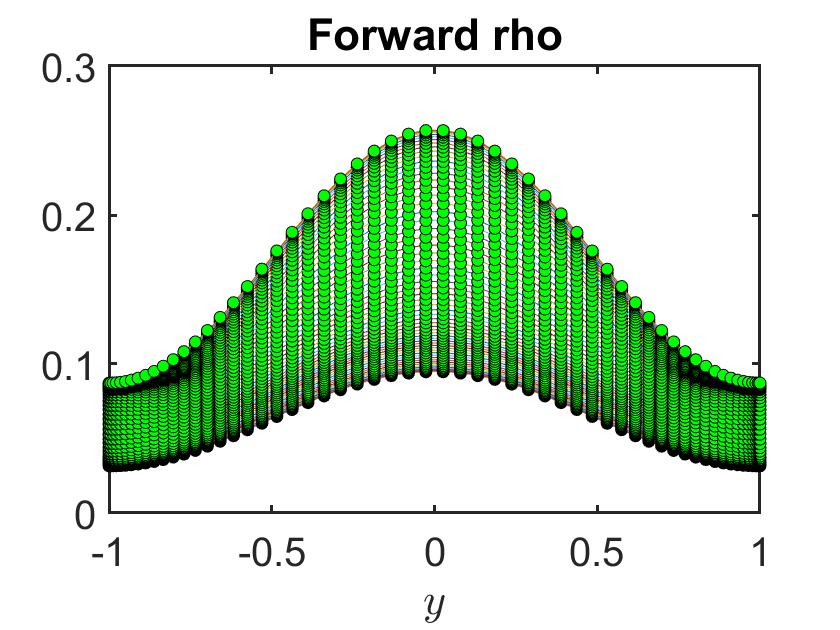
\includegraphics[scale=0.3]{wFrhoFW2.jpg}	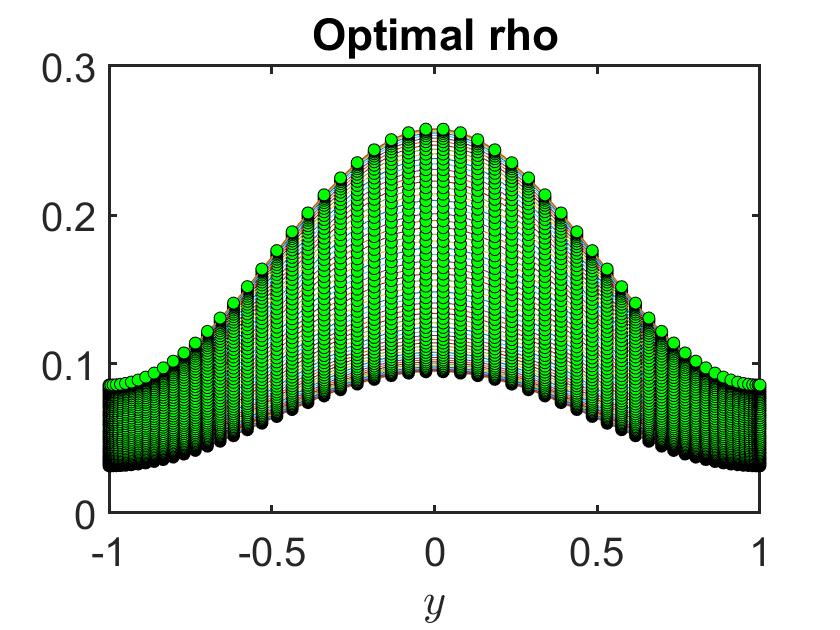
\includegraphics[scale=0.3]{wFrhoOpt2.jpg}
	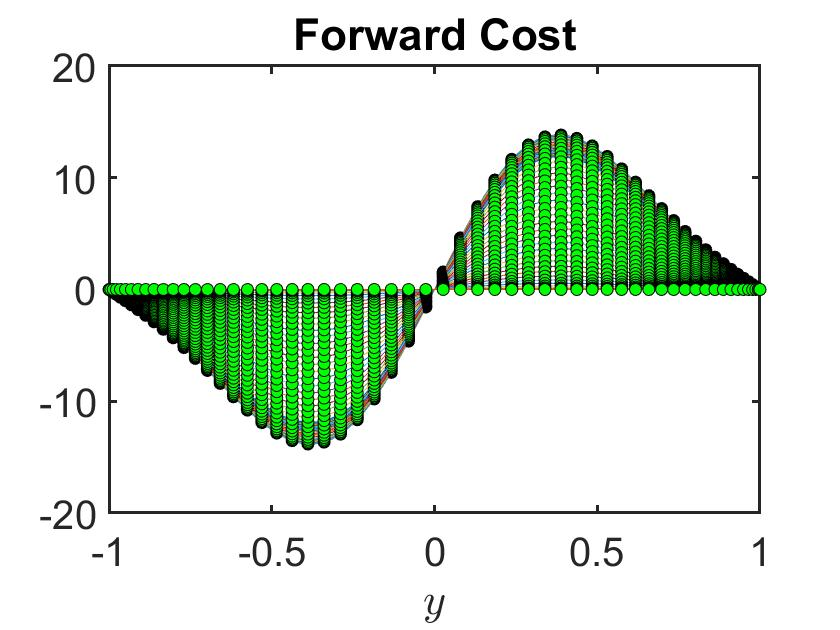
\includegraphics[scale=0.3]{wFwFW2.jpg}
	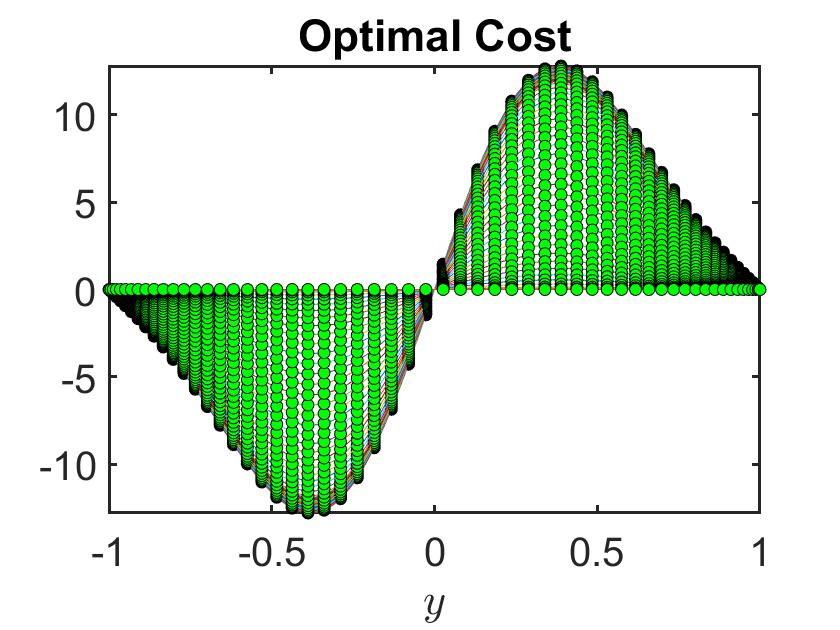
\includegraphics[scale=0.3]{wFwOpt2.jpg}
	\caption{Solutions $\rho_{FW}$ and $\rho_{Opt}$, $w_{FW}$ and $w_{Opt}$,   with $D_0 = 1$.}
	\label{rhoD032}
\end{figure}

\begin{figure}[h]
	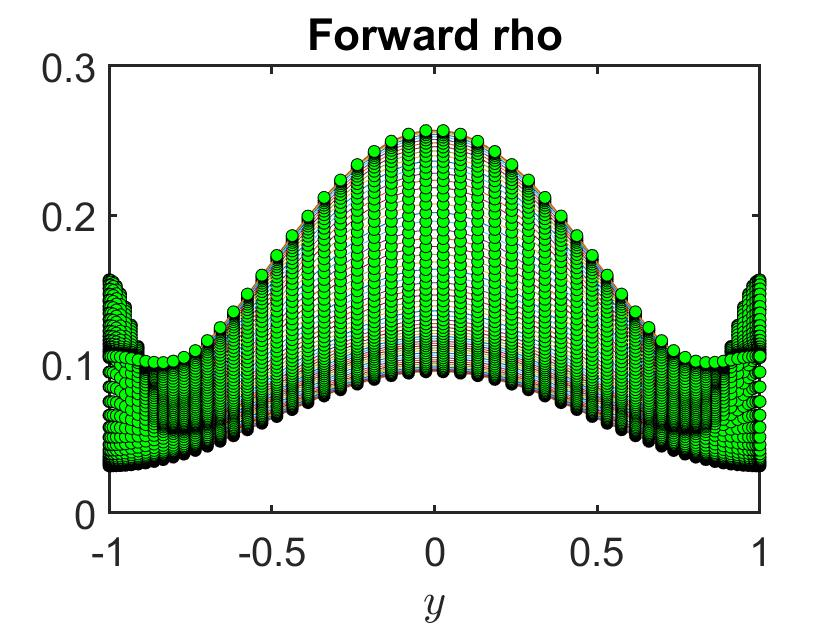
\includegraphics[scale=0.3]{wFrhoFW2a.jpg}	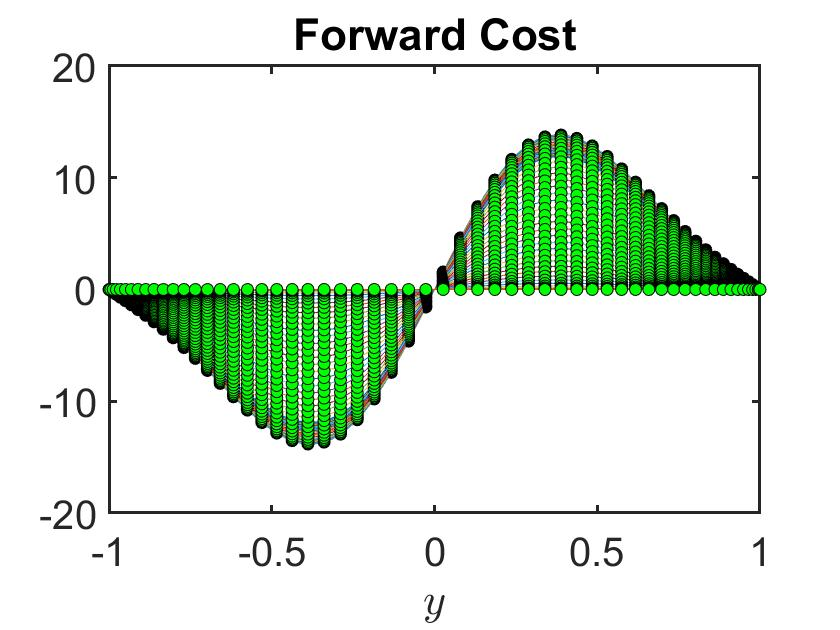
\includegraphics[scale=0.3]{wFwFW2a.jpg}
	\caption{Solutions $\rho_{FW}$ and $w_{FW}$,   with $D_0 = 0.1$.}
	\label{rhoD032a}
\end{figure}

\end{document}
